%
%  exercise-1.tex
%  artificial intelligence
%
%  Created by Illya Starikov on 01/17/18.
%  Copyright 2018. Illya Starikov. All rights reserved.
%

\RequirePackage[l2tabu, orthodox]{nag}
\documentclass[12pt]{scrartcl}

\newcommand{\exercisenumber}{1}
\newcommand{\duedate}{July 6\textsuperscript{th}, 2018}
\usepackage{amssymb,amsmath,verbatim,graphicx,microtype,upquote,units,booktabs,akkwidepage}

\newcommand{\chapterNumber}[1]{
    \setcounter{section}{#1}
    \addtocounter{section}{-1}
}

\begin{document}
\maketitle

\section{1-Rule Method}
\begin{statement}
    Use the 1-rule (1R) method to find the best single attribute to determine restaurant. In order to demonstrate that you actually know how this method works (and aren’t just guessing at which attribute is best), you must fill in ALL of the blank values in the table below; otherwise, you will not receive any credit for this problem.
\end{statement}

\begin{table}[H]
    \centering
    \resizebox{\columnwidth}{!}{%
        \begin{tabular}{l|l|l|l|l|l}
            \hline
            \multicolumn{1}{|l|}{\textbf{Attribute}} & \textbf{Attribute Value} & \textbf{\# Rows} & \textbf{Most Frequent Value} & \textbf{Errors} & \multicolumn{1}{l|}{\textbf{Total Errors}} \\ \hline
            \multicolumn{1}{|l|}{Meal Preference}    & Hamburger                & 3                                   & McDonalds (3)                               & 0               & \multicolumn{1}{l|}{2}                     \\ \hline
                                         & Fish                     & 2                                   & Burger King (2)                             & 0               &                                            \\ \cline{2-5}
                                         & Chicken                  & 4                                   & Wendy's (2)                                 & 2               &                                            \\ \hline
            \multicolumn{1}{|l|}{Gender}             & M                        & 5                                   & Burger King/McDonald's (2/2)                & 3               & \multicolumn{1}{l|}{5}                     \\ \hline
                                         & F                        & 4                                   & McDonald's (2)                              & 2               &                                            \\ \hline
            \multicolumn{1}{|l|}{Drink Preference}   & Pepsi                    & 3                                   & Burger King (2)                             & 1               & \multicolumn{1}{l|}{3}                     \\ \hline
                                         & Coke                     & 6                                   & McDonald's (4)                              & 2               &                                            \\ \cline{2-5}
        \end{tabular}
    }
\end{table}

From this, the following rules would be generated:
\begin{alignat*}{3}
    &\text{Meal Preference $=$ \textit{Hamburger}} &&\implies \text{McDonald's} \\
    &\text{Meal Preference $=$ \textit{Fish}}      &&\implies \text{Burger King} \\
    &\text{Meal Preference $=$ \textit{Chicken}}   &&\implies \text{Wendy's} \\
\end{alignat*}


\section{Decision Stump}
\begin{statement}
    Create the dataset given in problem 1. as an arff or csv file, and run DecisionStump on it in Weka. List the classification rules that are produced by Weka (you can just include a screenshot of your Weka output) AND hand-draw the decision tree that corresponds to those rules.
\end{statement}

From Weka's Decision Stump, we get the following output:

\begin{figure}[H]
    \centering
    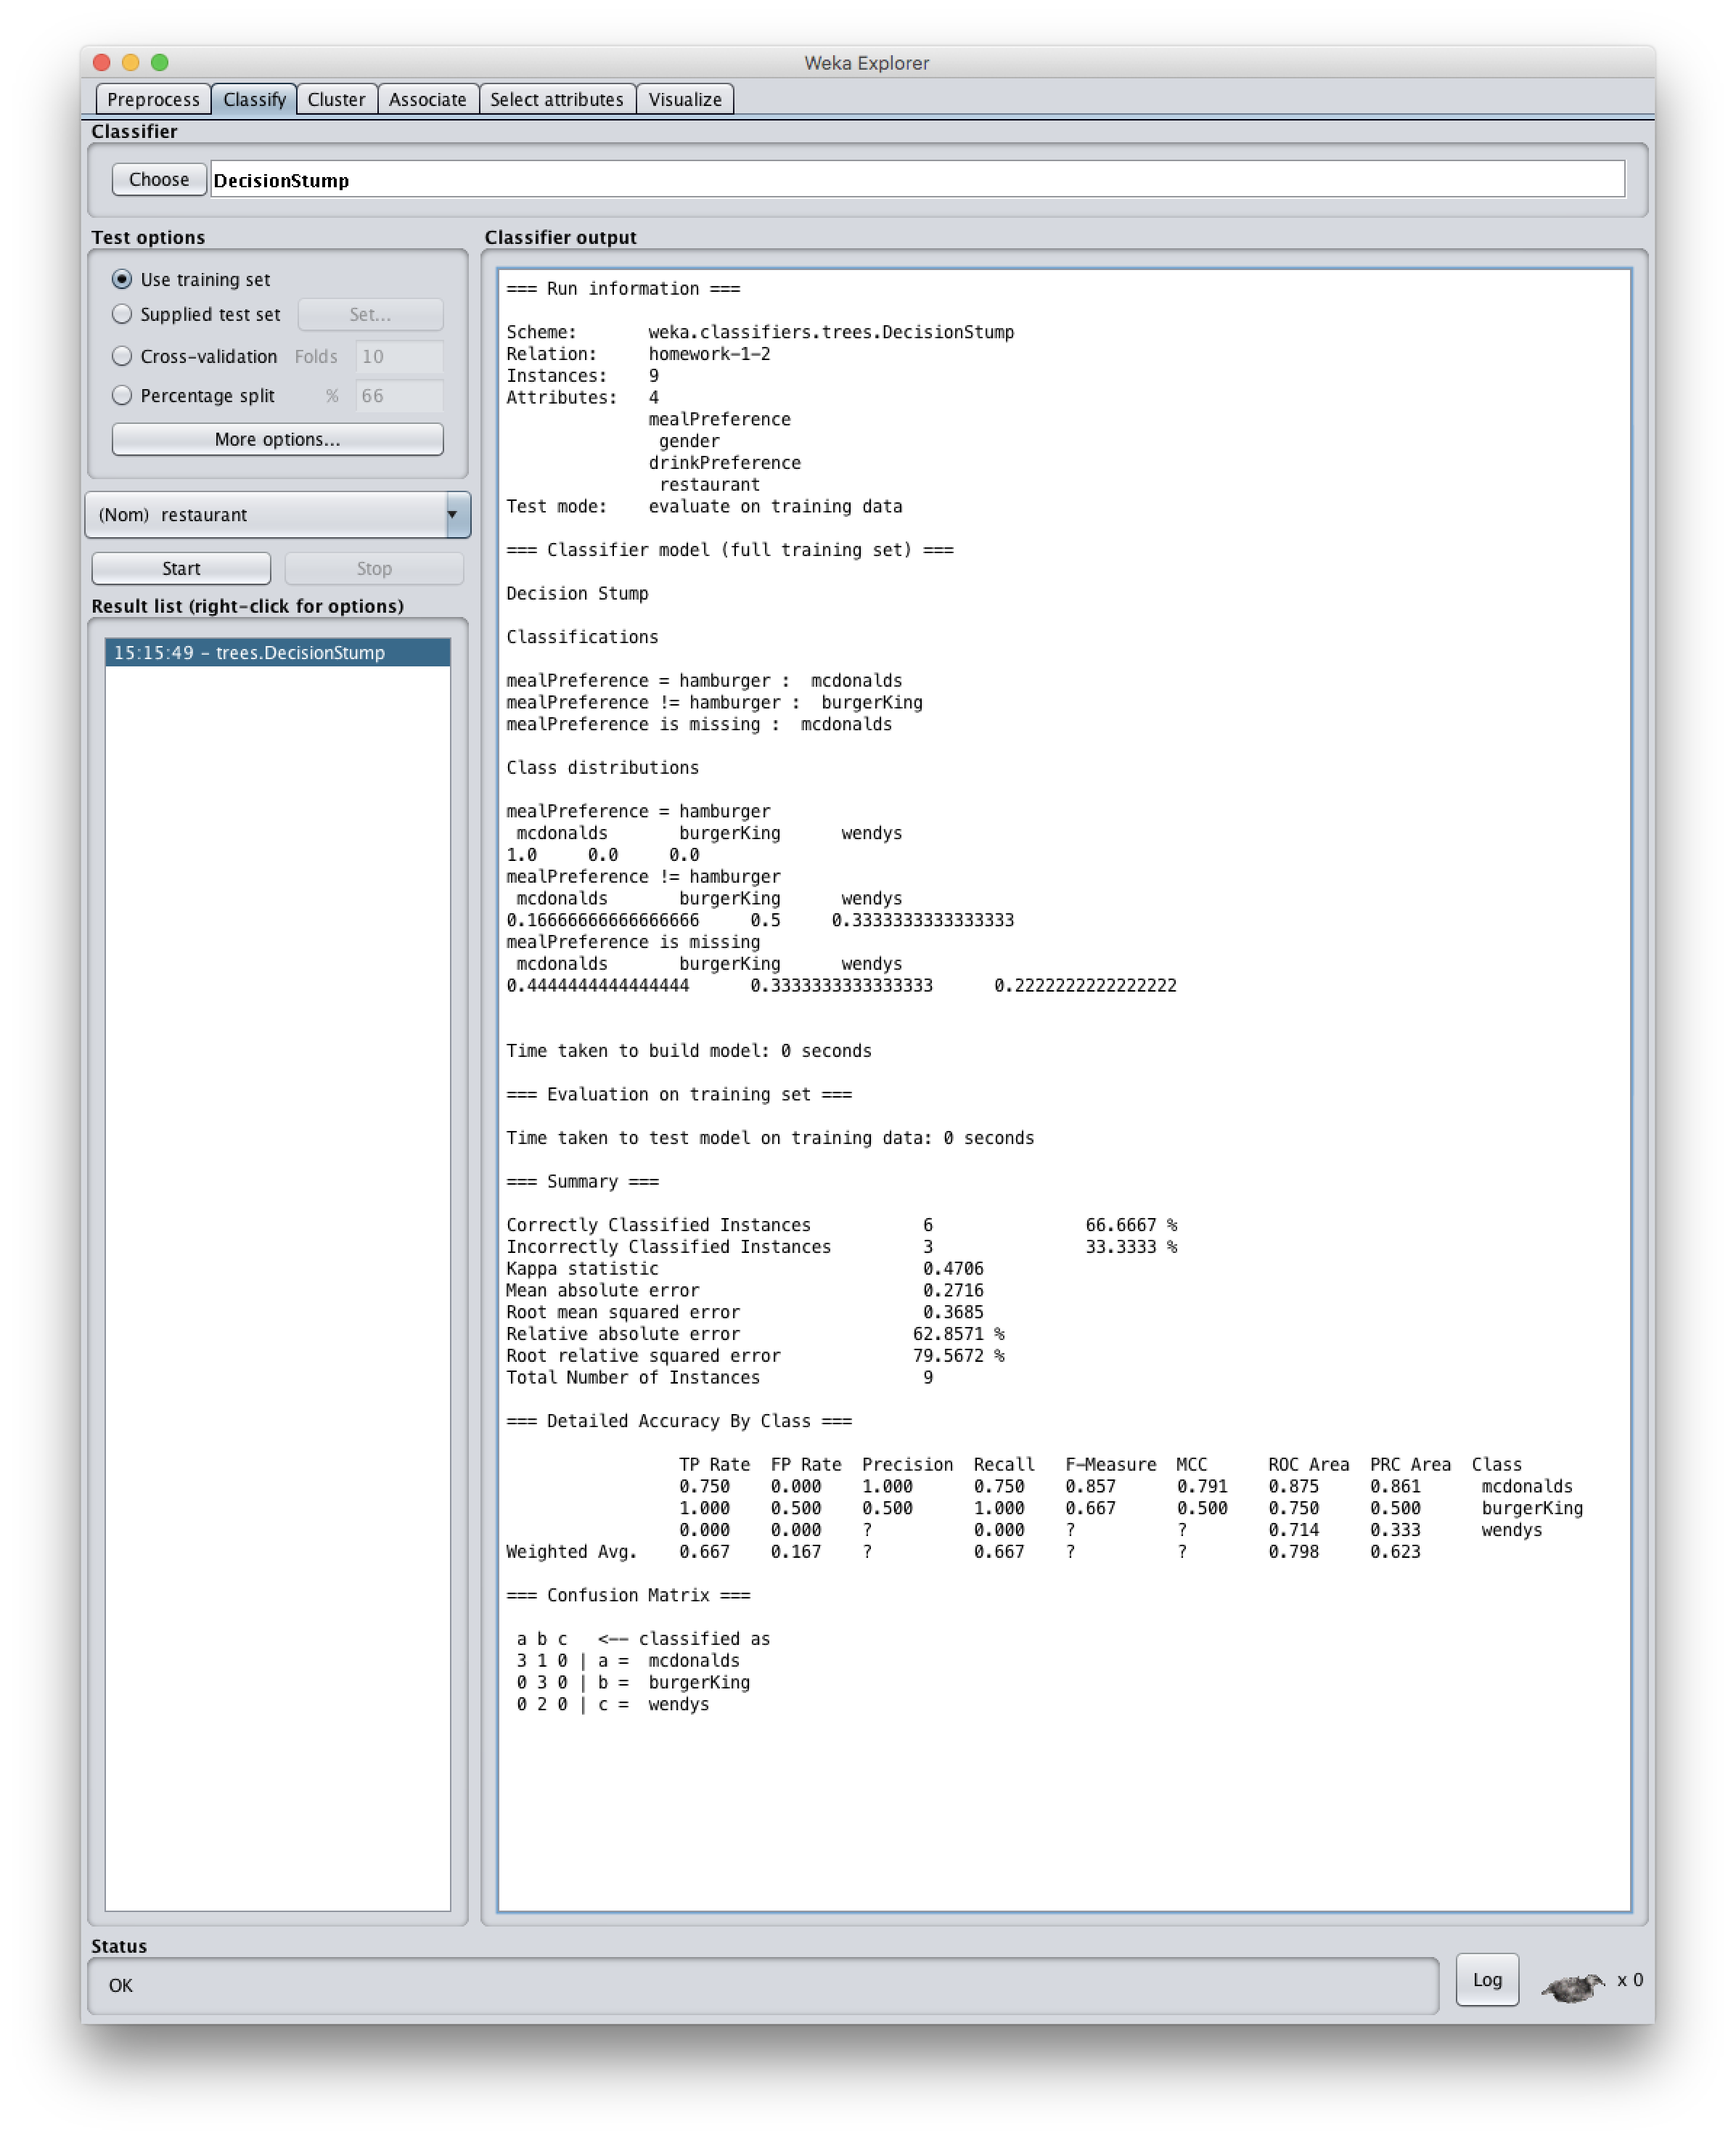
\includegraphics[width=.75\linewidth]{assets/problem-1.png}
    \label{fig:assets/homework-1-1}
\end{figure}

For the figure, we get the following decision tree:

\begin{center}
    \begin{forest}
        [Meal Preference
            [Is Hamburger
                [McDonald's]
            ]
            [Not Hamburger
                [Burger King]
            ]
            [Missing
                [McDonald's]
            ]
        ]
    \end{forest}
\end{center}

\section{Statistical Modeling}
\begin{statement}
    Statistical modeling can be used to compute the probability of occurrence of an attribute value. Based on the data given in the table below, if we have a new instance where ageGroup = youngAdult, gender = M, and bookPreference = nonFiction, what is the likelihood that musicPreference = country? Just set up the equation to compute this with the appropriate values; you don’t have to actually calculate the final answer.
\end{statement}

\begin{equation*}
    \text{Likelihood of Country} =
    \nicefrac{2}{3} \times
    \nicefrac{1}{3} \times
    \nicefrac{1}{3} \times
    \nicefrac{3}{8} = \nicefrac{1}{36} \approx 0.02\bar{7}
\end{equation*}


\section{Id3}
\begin{statement}
    Create the dataset given in problem 1. as an arff or csv file, and run Id3 on it in Weka. Include a screenshot of the decision tree output that is produced by Weka AND hand-draw the decision tree. Note: You may have to install the package containing Id3.
\end{statement}

From Weka's Id3, we get the following output:

\begin{figure}[H]
    \centering
    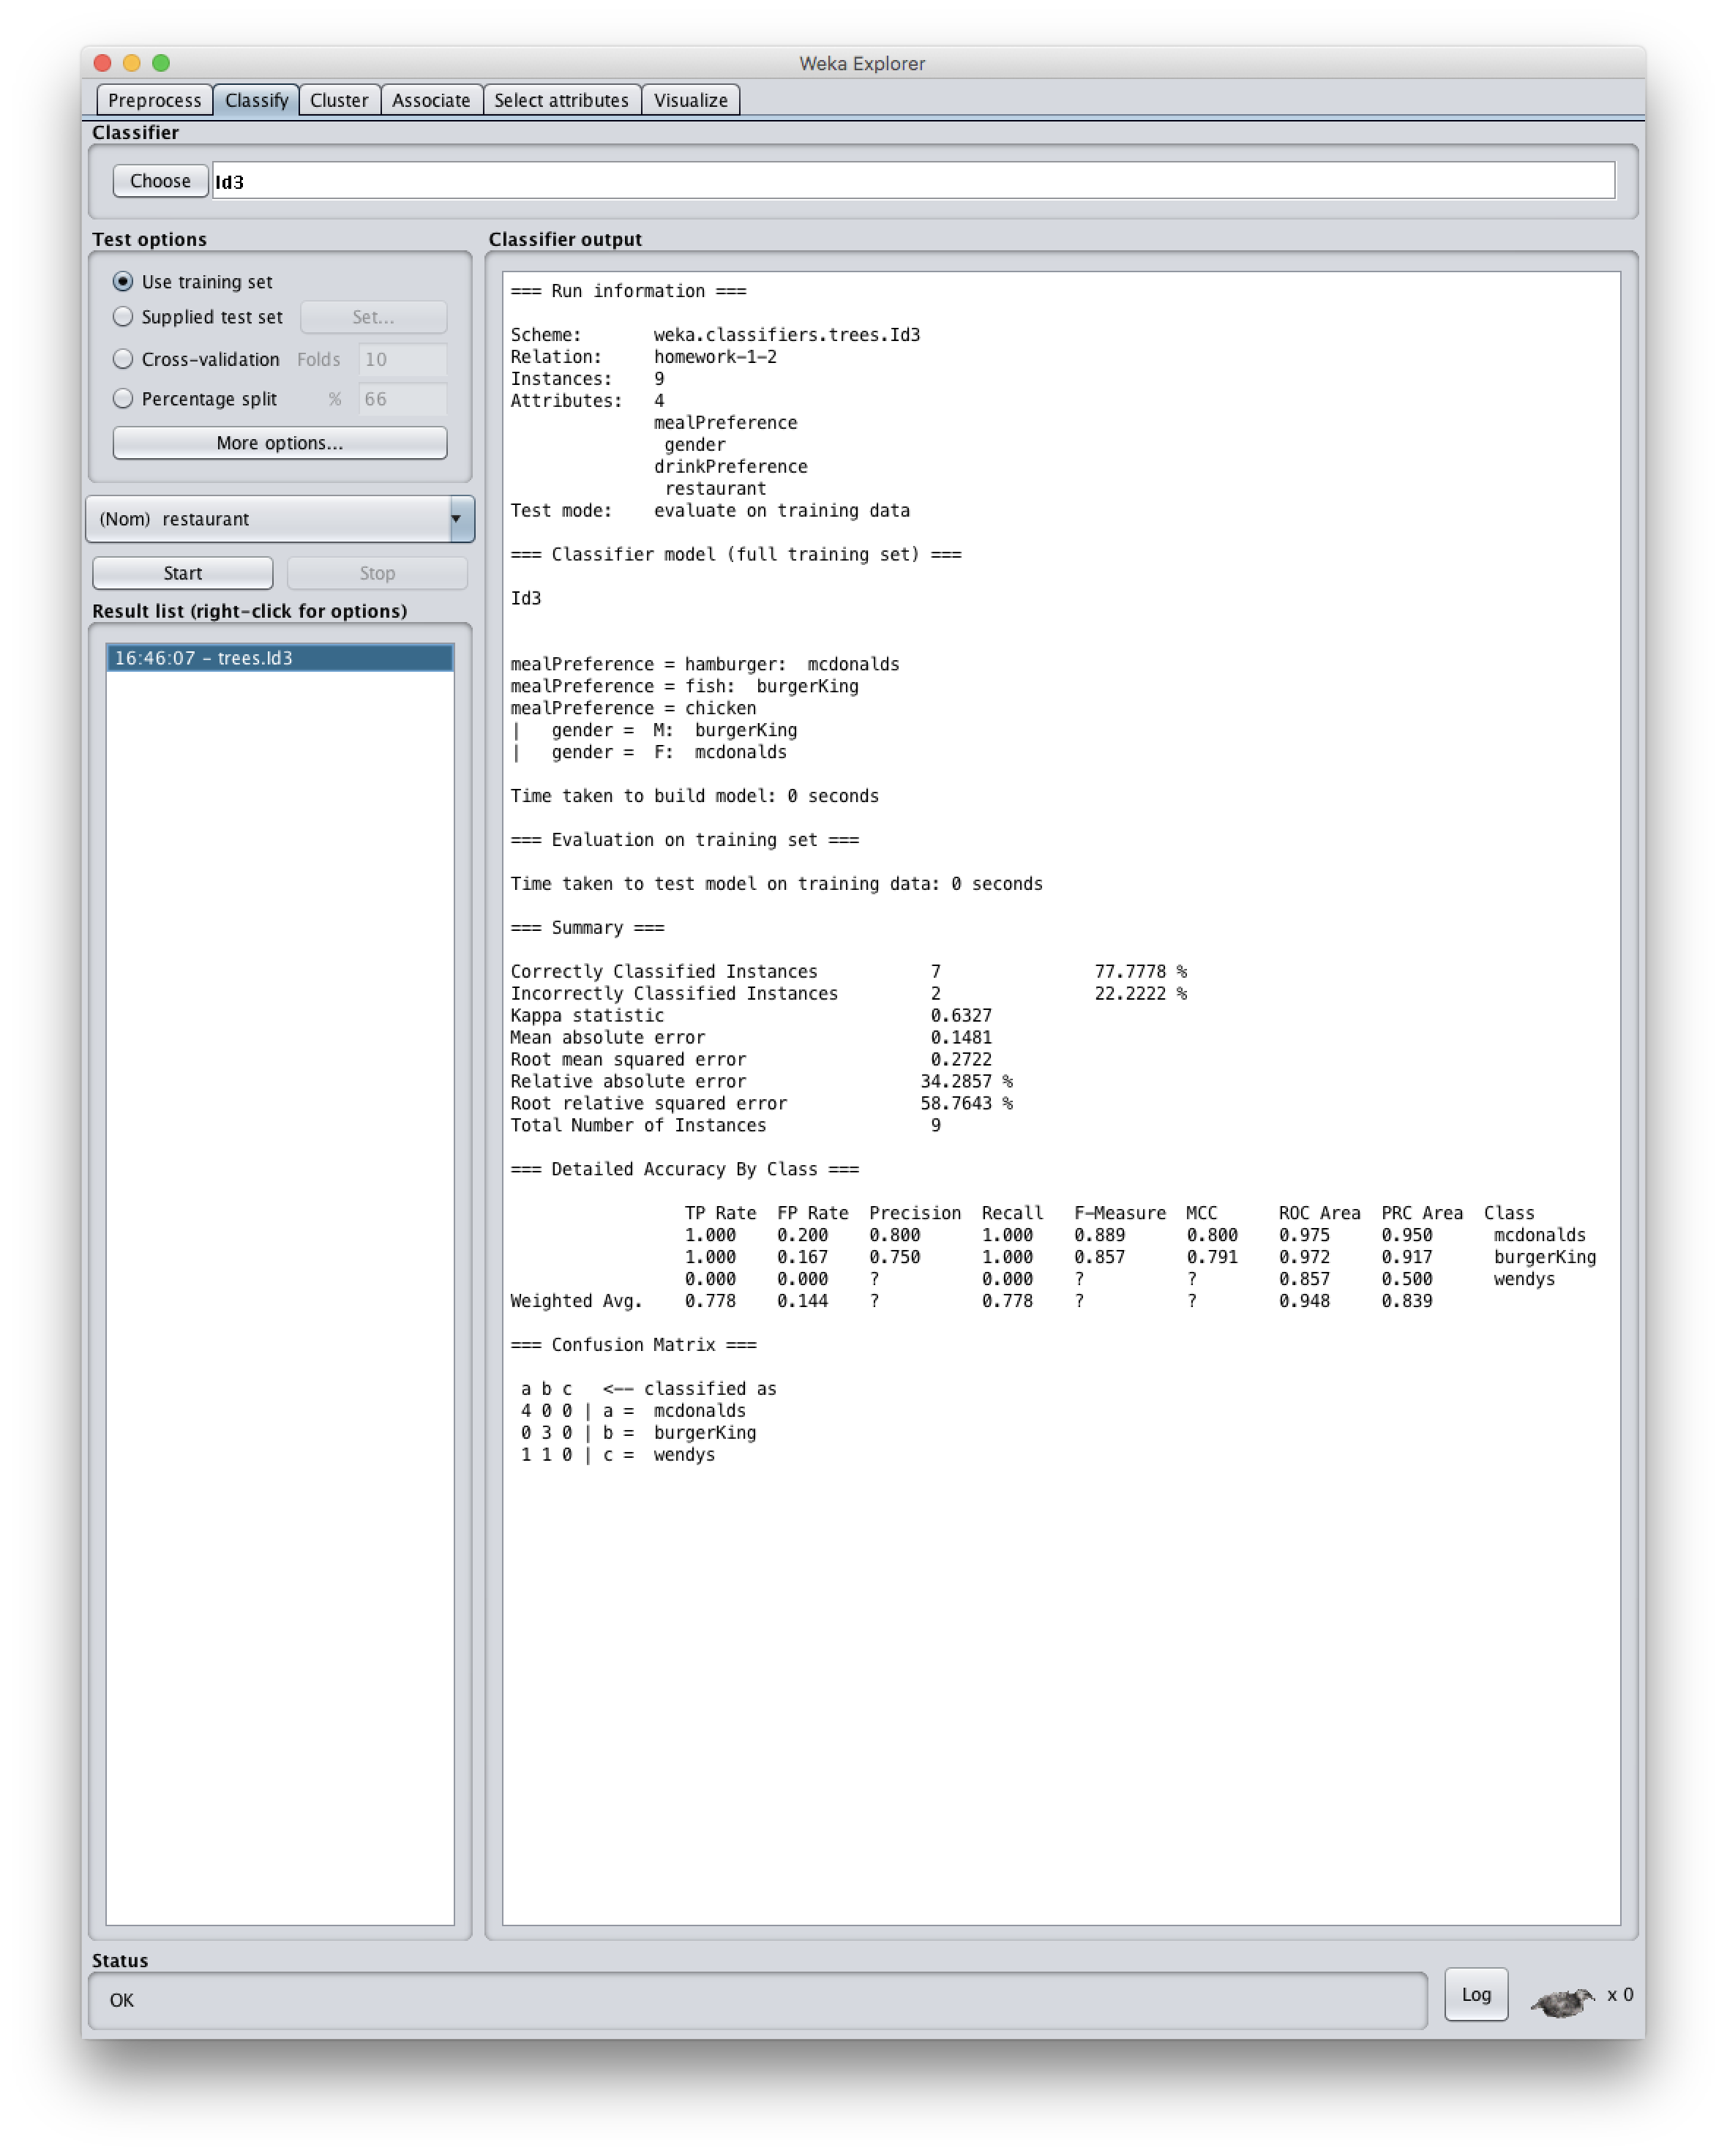
\includegraphics[width=.75\linewidth]{assets/problem-4.png}
    \label{fig:assets/homework-1-4}
\end{figure}

For the figure, we get the following decision tree:

\begin{center}
    \begin{forest}
        [Meal Preference
            [Hamburger
                [McDonald's]
            ]
            [Fish
                [Burger King]
            ]
            [Chicken
                [Male
                    [Burger King]
                ]
                [Female
                    [McDonald's]
                ]
            ]
        ]
    \end{forest}
\end{center}


\section{Entropy}
\begin{statement}
    If we want to make a decision tree for determining restaurant, we must decide which of the three non-decision attributes (mealPreference, gender, or drinkPreference) to use as the root of the tree.
\end{statement}

\begin{itemize}
    \item \textit{Set up the equation to compute what in lecture we called entropyBeforeSplit for restaurant. You do not have to actually solve (i.e., calculate the terms in) the equation, just set up the equation with the appropriate values.}
        \begin{equation*}
            \text{Entropy Before Split} =
            -\nicefrac{3}{10}\,\log_2\left(\nicefrac{3}{10}\right)
            - \nicefrac{5}{10}\,\log_2\left(\nicefrac{5}{10}\right)
            - \nicefrac{2}{10}\,\log_2\left(\nicefrac{2}{10}\right)
            \approx 1.485
        \end{equation*}


    \item \textit{Set up the equation to compute entropy for mealPreference when its value is chicken. That is, a tree with mealPreference at the root would have three branches (one for hamburger, one for chicken, and one for fish), requiring us to compute entropyHamburger, entropyChicken, and entropyFish; here we only want you to set up the equation to compute entropyChicken. You do not have to actually solve (i.e., calculate the terms in) the equation, just set it up using the appropriate values.}
        \begin{equation*}
            \text{Entropy Chicken} =
            -\nicefrac{1}{4}\,\log_2\left(\nicefrac{1}{4}\right)
            - \nicefrac{1}{4}\,\log_2\left(\nicefrac{1}{4}\right)
            - \nicefrac{2}{4}\,\log_2\left(\nicefrac{2}{4}\right)
            \approx 1.040
        \end{equation*}


    \item \textit{Suppose that instead of considering mealPreference to be the root of this decision tree, we had instead considered drinkPreference. Set up the equation to compute information gain for drinkPreference given the variables specified below.}
        \begin{equation*}
            \text{Information Gain} =
            X -
            \left(\nicefrac{7}{10}\, C + \nicefrac{3}{10}\, P\right)
        \end{equation*}


\end{itemize}


\section{isSticky}
\begin{statement}
    Create the dataset shown below as an arff or csv file and run the Prism algorithm on it in Weka specifying isSticky as the decision attribute. List the classification rules that are produced (you can just include a screenshot of your Weka output). Then work out the Prism algorithm by hand to show what classification rules you would get; who knows, they might be different!
\end{statement}

\subsection{Is Sticky = No}
\begin{table}[H]
    \centering
    \begin{tabular}{|l|l|l|l|l|}
        \hline
        \textbf{consistency} & \textbf{packaging}  & \textbf{chocolate} & \textbf{roundShaped} & \textbf{isSticky} \\ \hline
        \textbf{soft}        & individuallyWrapped & yes                & no                   & no \\
        \textbf{soft}        & box                 & yes                & no                   & no \\
        \textbf{hard}        & sack                & no                 & yes                  & no \\
        \textbf{hard}        & box                 & yes                & yes                  & no \\
        \textbf{hard}        & individuallyWrapped & no                 & no                   & yes \\
        \textbf{hard}        & box                 & no                 & yes                  & yes \\
        \textbf{soft}        & individuallyWrapped & no                 & no                   & yes \\\hline
    \end{tabular}
\end{table}

Which leads us to the following $T$ and $P$ values:

\subsection{Is Sticky = No}
\begin{table}[H]
    \centering
    \begin{tabular}{|l|c|c|c|}
        \hline
        \texbf{Label}                 & $T$ & $P$ & $T/P$ \\\hline
        \textbf{soft}                 & 3   & 2   & 0.66\\
        \textbf{hard}                 & 4   & 2   & 0.50\\
        \textbf{individually wrapped} & 3   & 1   & 0.33\\
        \textbf{box}                  & 3   & 2   & 0.66\\
        \textbf{sack}                 & 1   & 1   & 1\\
        \textbf{chocolate}            & 3   & 3   & 1\\
        \textbf{not chocolate}        & 4   & 1   & 0.25\\
        \textbf{round}                & 3   & 2   & 0.66\\
        \textbf{not round}            & 4   & 2   & 0.5\\\hline
    \end{tabular}
\end{table}

This leads to the following rule:

\begin{equation*}
    \text{chocolate = yes} \implies \text{is sticky = no}
\end{equation*}

Reducing Our dataset to:

\subsection{Is Sticky = No}
\begin{table}[H]
    \centering
    \begin{tabular}{|l|l|l|l|l|}
        \hline
        \textbf{consistency} & \textbf{packaging}  & \textbf{chocolate} & \textbf{roundShaped} & \textbf{isSticky} \\\hline
        \textbf{hard}        & sack                & no                 & yes                  & no \\
        \textbf{hard}        & individuallyWrapped & no                 & no                   & yes \\
        \textbf{hard}        & box                 & no                 & yes                  & yes \\
        \textbf{soft}        & individuallyWrapped & no                 & no                   & yes \\\hline
    \end{tabular}
\end{table}

Which leads us to the following $T$ and $P$ values:

\subsection{Is Sticky = No}
\begin{table}[H]
    \centering
    \begin{tabular}{|l|l|l|l|l|}
        \hline
        \textbf{consistency} & \textbf{packaging}  & \textbf{chocolate} & \textbf{roundShaped} & \textbf{isSticky} \\\hline
        \textbf{hard}        & sack                & no                 & yes                  & no \\
        \textbf{hard}        & individuallyWrapped & no                 & no                   & yes \\
        \textbf{hard}        & box                 & no                 & yes                  & yes \\
        \textbf{soft}        & individuallyWrapped & no                 & no                   & yes \\\hline
    \end{tabular}
\end{table}

Which leads us to the following $T$ and $P$ values:

\begin{table}[H]
    \centering
    \begin{tabular}{|l|c|c|c|}
        \hline
        \texbf{Label}                 & $T$ & $P$ & $T/P$ \\\hline
        \textbf{soft}                 & 1   & 0   & 0 \\
        \textbf{hard}                 & 3   & 1   & 0.33 \\
        \textbf{individually wrapped} & 2   & 0   & 0 \\
        \textbf{box}                  & 1   & 0   & 0 \\
        \textbf{sack}                 & 1   & 1   & 1 \\
        \textbf{chocolate}            & 0   & 0   & \\
        \textbf{not chocolate}        & 4   & 1   & 0.25 \\
        \textbf{round}                & 2   & 1   & 0.5 \\
        \textbf{not round}            & 2   & 0   & 0 \\\hline
    \end{tabular}
\end{table}

Which leads us to the following rule:

\begin{equation*}
    \text{packaging = sack} \implies \text{is sticky = no}
\end{equation*}


\subsection{Is Sticky = Yes}
\begin{table}[H]
    \centering
    \begin{tabular}{|l|l|l|l|l|}
        \hline
        \textbf{hard} & \textbf{individuallyWrapped} & \textbf{no} & \textbf{no} & \textbf{yes} \\\hline
        \textbf{hard} & box                          & no          & yes         & yes \\
        \textbf{soft} & individuallyWrapped          & no          & no          & yes \\\hline
    \end{tabular}
\end{table}

Which leads us to the following $T$ and $P$ values:

\subsection{Is Sticky = No}
\begin{table}[H]
    \centering
    \begin{tabular}{|l|c|c|c|}
        \hline
        \texbf{Label}                 & $T$ & $P$ & $T/P$ \\\hline
        \textbf{soft}                 & 1   & 1   & 1 \\
        \textbf{hard}                 & 2   & 2   & 1 \\
        \textbf{individually wrapped} & 2   & 2   & 1 \\
        \textbf{box}                  & 1   & 1   & 1 \\
        \textbf{sack}                 & 0   & 0   & \\
        \textbf{chocolate}            & 0   & 0   & \\
        \textbf{not chocolate}        & 3   & 3   & 1 \\
        \textbf{round}                & 1   & 1   & 1 \\
        \textbf{not round}            & 2   & 2   & 1 \\\hline
    \end{tabular}
\end{table}

Which leads us to the following rule:

\begin{equation*}
    \text{chocolate = no} \implies \text{is sticky = yes}
\end{equation*}

\subsection{Final Ruleset}
From this, the following rules would be generated:
\begin{alignat*}{3}
    &\text{chocolate = yes}  &&\implies \text{is sticky = no} \\
    &\text{packaging = sack} &&\implies \text{is sticky = no} \\
    &\text{chocolate = no}   &&\implies \text{is sticky = yes}
\end{alignat*}

\subsection{Weka Output}
\begin{figure}[H]
    \centering
    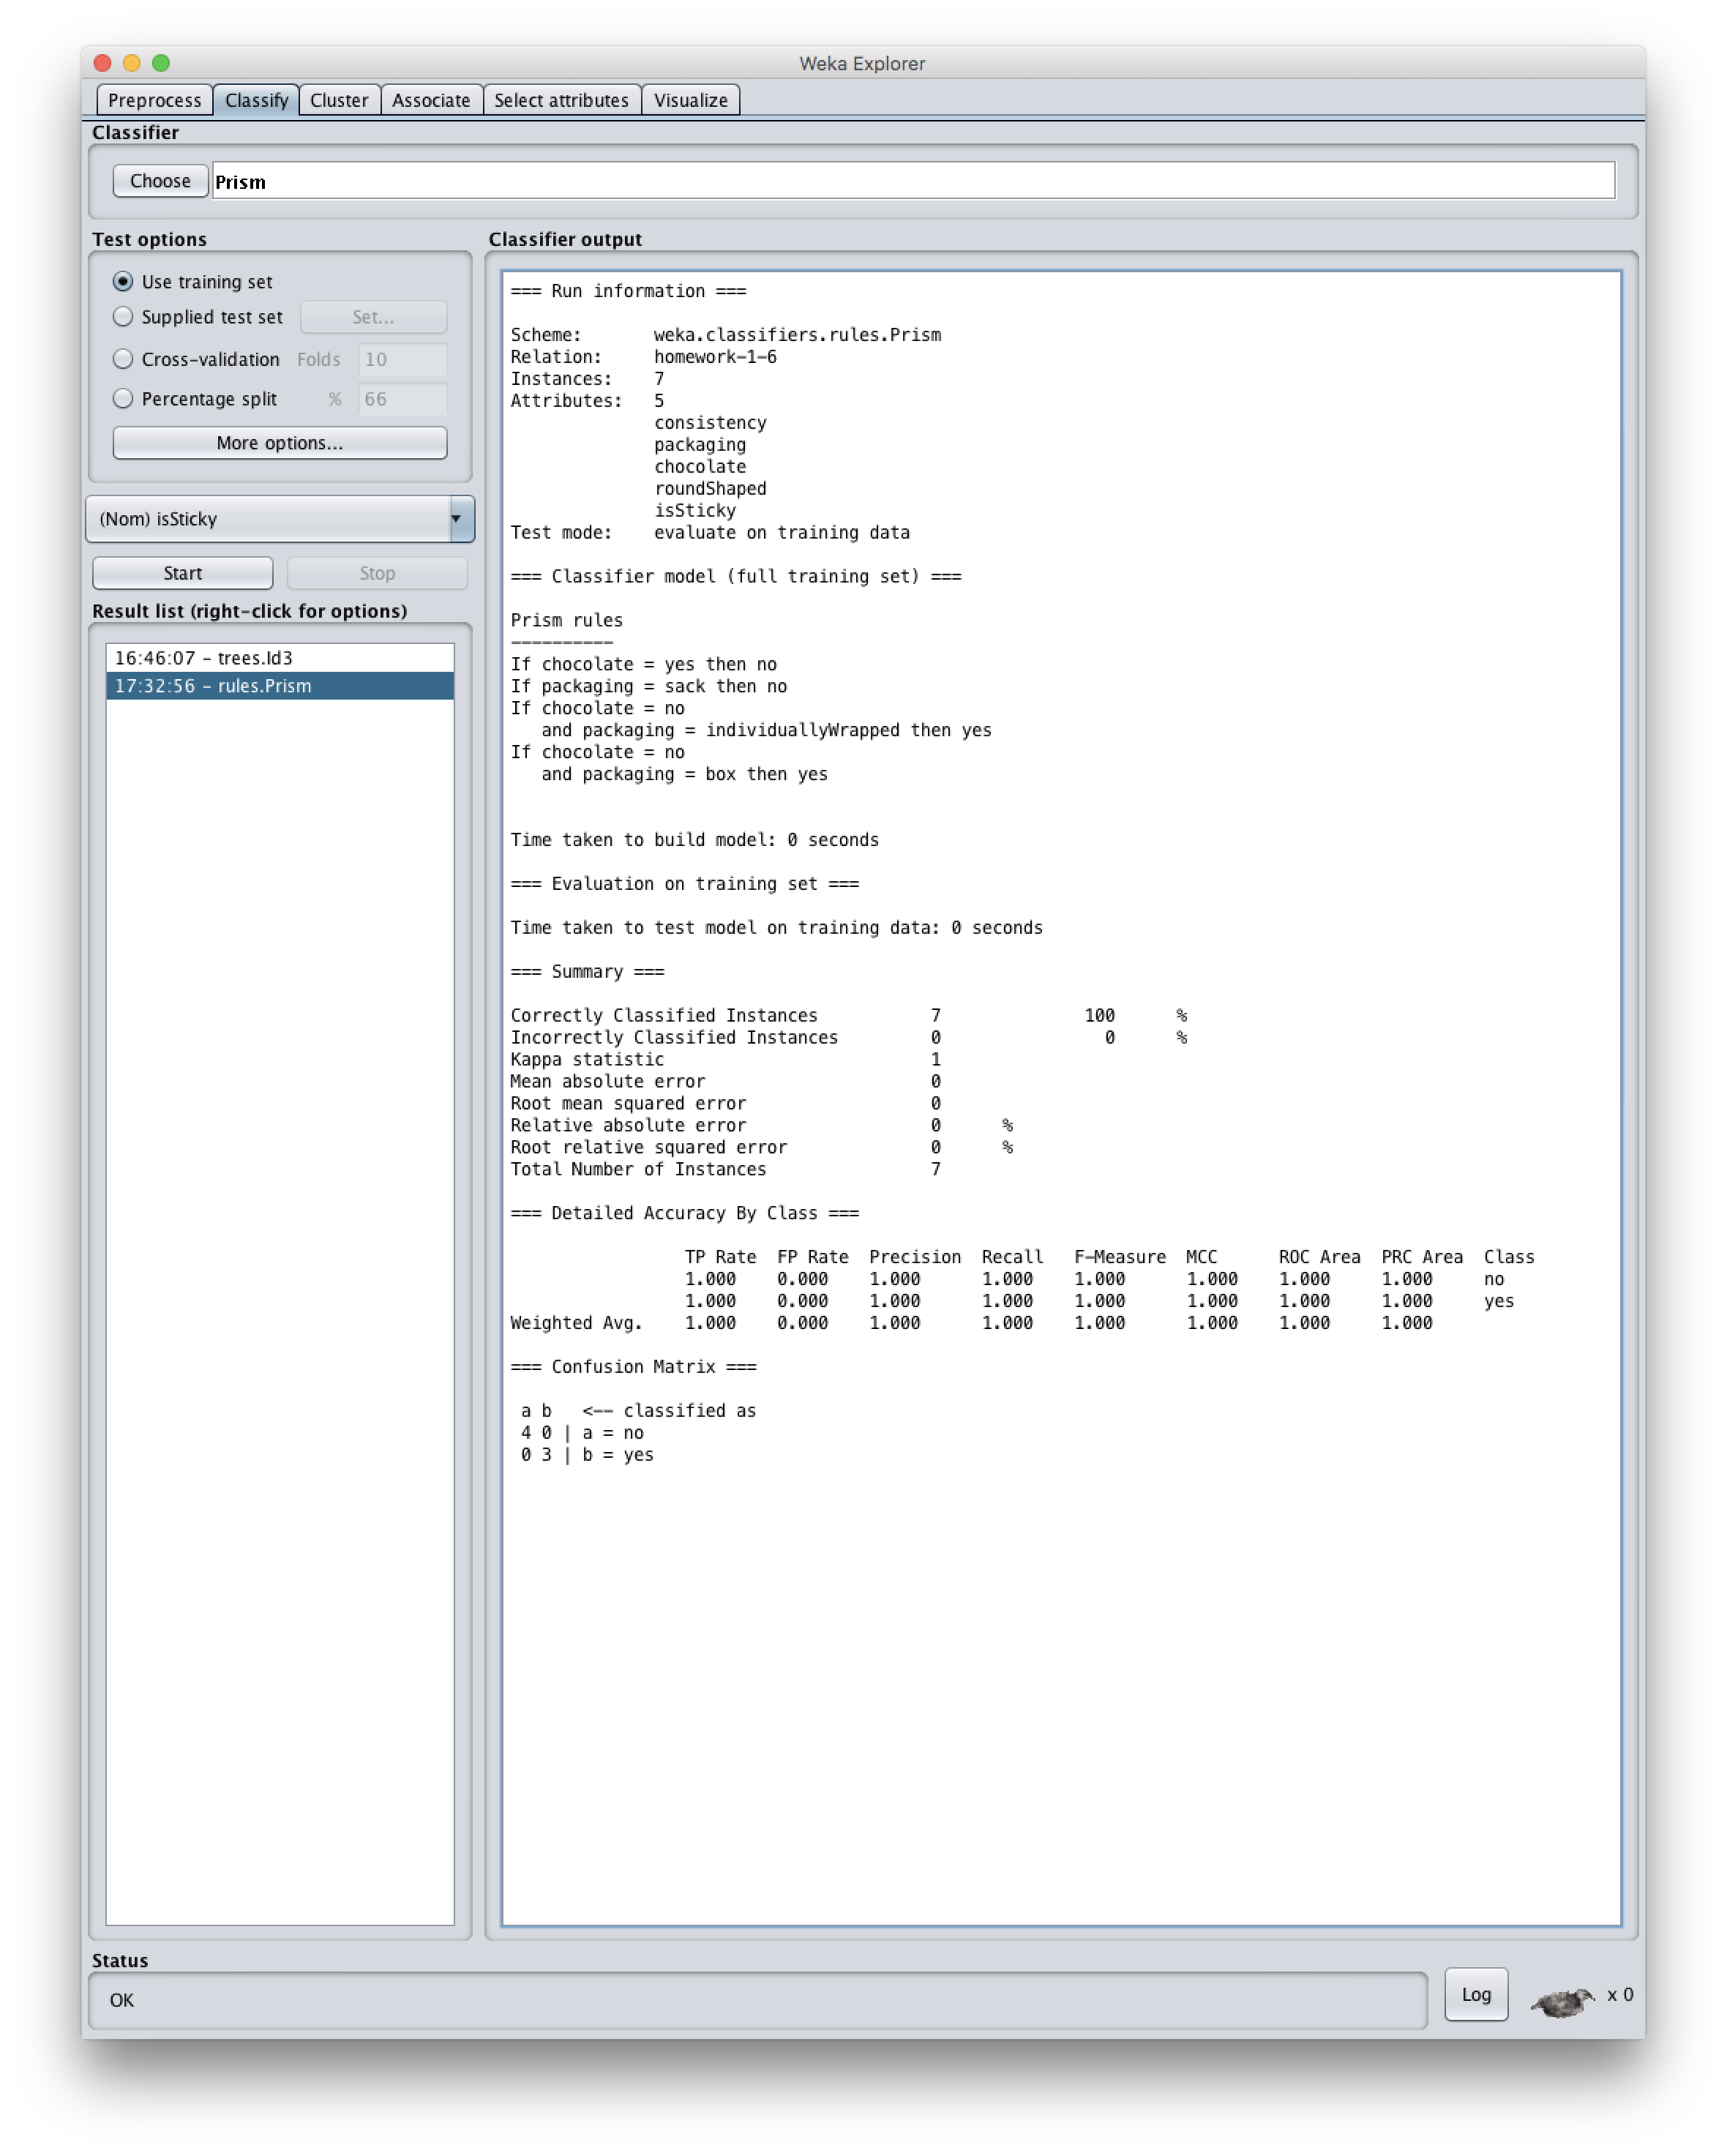
\includegraphics[width=.75\linewidth]{assets/problem-6.png}
    \label{fig:assets/homework-1-6}
\end{figure}
\end{document}
